\section{Strategie}

Testowanie na podstawie właściwości nie jest proste w zastosowaniu, przynajmniej przy pierwszej próbie.
Istnieją jednak pewne schematy wskazujące drogę, jak stworzyć takie testy.
\subsection{Różne ścieżki, ten sam wynik}

Jedną z podstawowych strategii skorzystanie z komutatywności niektórych operacji. Można to zrobić poprzez wykonanie operacji w różnej kolejności, jak zaprezentowano w \refrys{fig:commutative_strategy}.
\begin{figure}[h]
    \centering
    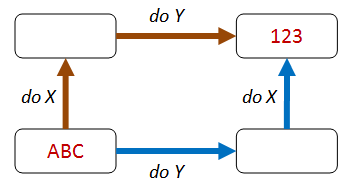
\includegraphics[width=0.5\textwidth]{images/property_commutative.png}
    \caption{Strategia - komutatywność}
    \label{fig:commutative_strategy}
\end{figure}

Przykładem takiej strategii może być komutatywność dodawania z \reflist{kod:add_all_properties}, gdzie wykorzystano \texttt{add x y}, jak i odwrotność tej operacji \texttt{add y x}. 
Innym przykładem jest test metody \texttt{sort} danej listy. 
Wykonanie sortowania, a następnie dodanie do każdego elementu listy \texttt{1} powinno dać taki sam efekt jak dodanie \texttt{1} do każdego z elementów listy, a następnie jej posortowanie \refrys{fig:commutative_strategy_list_sort} \reflist{kod:list_sort_add1}.

\begin{figure}
    \centering
    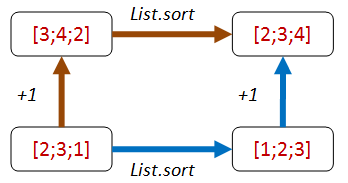
\includegraphics[width=0.5\textwidth]{images/property_list_sort1.png}
    \caption{Strategia - komutatywność - sortowanie listy}
    \label{fig:commutative_strategy_list_sort}
\end{figure}
\lstset{language=FSharp, basicstyle=\scriptsize}
\begin{lstlisting}[frame=single,caption={Test sortowania listy z wykorzystaniem strategii komutatywnej},label=kod:list_sort_add1]
    let addThenSort_eq_sortThenAdd sortFn aList =
        let add1 x = x + 1

        let result1 = aList |> sortFn |> List.map add1
        let result2 = aList |> List.map add1 |> sortFn
        result1 = result2
\end{lstlisting}
Alternatywną formę tej strategi przedstawiono w \refrys{fig:commutative_strategy_list_sort_with_negation}
\begin{figure}
    \centering
    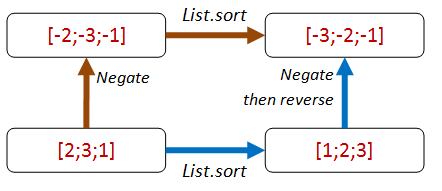
\includegraphics[width=0.5\textwidth]{images/property_list_sort3.png}
    \caption{Strategia - komutatywność - sortowanie listy z negacją}
    \label{fig:commutative_strategy_list_sort_with_negation}
\end{figure}

\subsection{Tam i z powrotem}

Test z wykorzystaniem inwersji \refrys{fig:inverse_strategy}, polega na sprawdzeniu, czy po zaaplikowaniu testowanej funkcji, następnie wykorzystaniu funkcji odwrotnej do otrzymania początkowych wartości.   
\begin{figure}
    \centering
    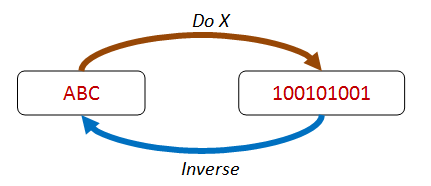
\includegraphics[width=0.5\textwidth]{images/property_inverse.png}
    \caption{Strategia - inwersja}
    \label{fig:inverse_strategy}
\end{figure}
Przykładem takiego testu mogą być przeciwne operacje matematyczne jak:
\begin{itemize}
    \item \texttt{dodawanie/odejmowanie}
    \item \texttt{mnożenie/dzielenie}
    \item \texttt{potęga/logarytm}.
\end{itemize} 
Innymi przykładami są operacje niekoniecznie matematyczne:
\begin{itemize}
    \item \texttt{serializacja/deserializacja}
    \item \texttt{zapis/odczyt z pliku}
    \item \texttt{wstaw/sprawdź czy zawiera}.
    \item \texttt{odwrócenie listy/odwrócenie listy} - \refrys{fig:inverse_strategy_list_inversion}
\end{itemize}

\begin{figure}
    \centering
    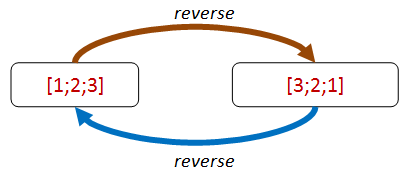
\includegraphics[width=0.5\textwidth]{images/property_list_rev_inverse.png}
    \caption{Strategia - inwersja - przykład}
    \label{fig:inverse_strategy_list_inversion}
\end{figure}

\subsection{Są rzeczy niezmienne}

Czasami testowana funkcja przetwarzając dane zachowuje część ich właściwości \refrys{fig:invariant_strategy}. 
Chociażby funkcje \texttt{sort} lub \texttt{map} wykonane na liście \texttt{n} elementów, zwracaja odpowiednio zmodyfikowaną listę \texttt{n} elementową \refrys{fig:invariant_strategy_example}.

\begin{figure}
    \centering
    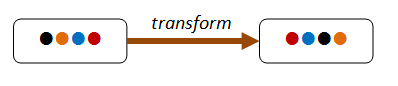
\includegraphics[width=0.5\textwidth]{images/property_invariant.png}
    \caption{Strategia - niezmienność}
    \label{fig:invariant_strategy}
\end{figure}

\begin{figure}
    \centering
    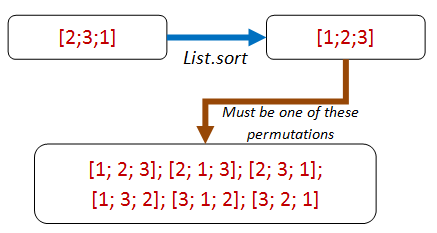
\includegraphics[width=0.5\textwidth]{images/property_list_sort_permutation.png}
    \caption{Strategia - niezmienność - przykład}
    \label{fig:invariant_strategy_example}
\end{figure}

\subsection{Z czasem rzeczy przestają się zmieniać}

Inną właściwością funkcji może być niezmienność wyniku funkcji po ponownym jej zaaplikowaniu \refrys{fig:independance_strategy}. 
Innymi słowy, wykonanie funkcji 2 razy daje taki sam efekt, jak jednokrotne jej zaaplikowanie.

\begin{figure}
    \centering
    
\includegraphics[width=0.5\textwidth]{images/property_idempotence.png}
    \caption{Strategia - idempotentność}
    \label{fig:independance_strategy}
\end{figure}

Przykładami takich operacji, dla których taki typ testu miałby zastosowanie to metoda \texttt{distinct} wykonana na danej liście, lub wykonanie \texttt{update} na danej bazie danych.

\subsection{Dziel i rządź}

Istnieją sposoby na testowanie na podstawie właściwości jest wykorzystanie rekursywności struktur przekazywanych do funkcji, takich jak \texttt{listy}, \texttt{drzewa} \refrys{fig:recursive_strategy}. 
Przykładem może być sprawdzenie za pomocą tej metody funkcji sort \reflist{kod:list_sort_rec}.

\begin{figure}
    \centering
    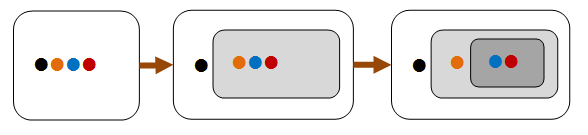
\includegraphics[width=0.5\textwidth]{images/property_induction.png}
    \caption{Strategia - rekursywność}
    \label{fig:recursive_strategy}
\end{figure}

\lstset{language=FSharp, basicstyle=\scriptsize}
\begin{lstlisting}[frame=single,caption={Test sortowania listy z wykorzystaniem strategii rekursywnej},label=kod:list_sort_rec]
let rec firstLessThanSecond_andTailIsSorted sortFn (aList:int list) =
  let sortedList = aList |> sortFn
  match sortedList with
  | [] -> true
  | [first] -> true
  | [first;second] -> first <= second
  | first::second::rest->
    first <= second &&
    let tail = second::rest
    // check that tail is sorted
    firstLessThanSecond_andTailIsSorted sortFn tail
\end{lstlisting}

\subsection{Łatwiej zweryfikować niż zaimplementować}
Niekiedy testowana funkcja jest skomplikowana, ale jej rezultat da się łatwo sprawdzić. Przykładem może być funkcja wyszukująca wyjście z labiryntu \refrys{fig:easy_verification_strategy}, gdzie sam algorytm wyszukiwania odpowiedniej ścieżki jest skomplikowany, 
natomiast samo sprawdzenie, czy ścieżka dobrze prowadzi do wyjścia można w łatwy sposób zweryfikować. Przykład użycia można zobaczyć w \refrys{fig:easy_verification_strategy_example} i~\reflist{kod:list_string_split}.

\begin{figure}
    \centering
    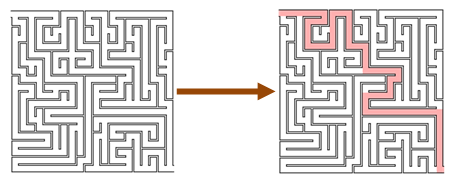
\includegraphics[width=0.5\textwidth]{images/property_easy_verification.png}
    \caption{Strategia - łatwe sprawdzenie}
    \label{fig:easy_verification_strategy}
\end{figure}

\begin{figure}
    \centering
    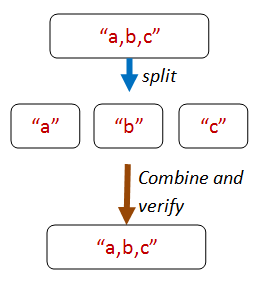
\includegraphics[width=0.35\textwidth]{images/property_string_split.png}
    \caption{Strategia - łatwe sprawdzenie - przykład \reflist{kod:list_string_split}}
    \label{fig:easy_verification_strategy_example}
\end{figure}

\lstset{language=FSharp, basicstyle=\scriptsize}
\begin{lstlisting}[frame=single,caption={Test string split},label=kod:list_string_split]
let concatElementsOfSplitString_eq_originalString (strings:string list) =
    // make a string
    let inputString = strings |> String.concat ","
    
    // use the 'split' function on the inputString
    let tokens = stringSplit inputString
    
    // build a string from the tokens
    let recombinedString = tokens |> String.concat ","
    
    // compare the result with the original
    inputString = recombinedString
\end{lstlisting}

\subsection{Testowanie z wyrocznią}

Zdaża się, że funkcjonalność została już napisana i trzeba ją zrefactorować, przepisać, napisać od nowa \refrys{fig:oracle_strategy}. Warto wtedy wykorzystać wartości zwracane przez oryginalnie zaimplementowany algorytm jako pewną wartość wyniku, pewnego rodzaju wyrocznię, uznając go jako prawdę. 
W taki sposób można sprawdzić, czy nowa funkcja w pewnym stopniu pokrywa się ze starą funkcją. Czasami też istnieje wiele algorytmów doprowadzających do tego samego wyniku, mające różne złożoności, czy też działające równolegle. 
Można wykożystać wtedy najprostrzy algorytm jako wyrocznię, ze względu na najmniejsze prawdopodobieństwo napisania takiego algorytmu z błędem. Następnie, przy wykorzystaniu wyroczni, stworzyć bardziej skomplikowany (często efektywniejszy) algorytm.

\begin{figure}
    \centering
    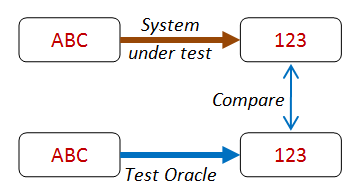
\includegraphics[width=0.5\textwidth]{images/property_test_oracle.png}
    \caption{Strategia - wyrocznia}
    \label{fig:oracle_strategy}
\end{figure}


